
\section{Eigenvalues and eigenvectors}
Start considering a generic square matrix $n \times n$. We are going later to discuss even the simmetry and positive definite properties.
Here below are the vectorial and the matrix form of the eigenvalue problem:
\[
    A\underline{x_i} = \lambda_i\underline{x_i} \hspace{0.5cm} i = 1, \dots, n \hspace{1cm} X^{-1}AX = \Lambda
\]
Where in the right-hand side there is a diagonal matrix $\Lambda$ with the eigenvalues of $A$ on the diagonal while the matrix $X$ with the eigenvectors of $A$ as columns.\\

\subsection*{Eigenvectors of matrix power}
What can we say about the eigenvectors and eigenvalues of $A^2$?
\[
    A^2\underline{x_i} = A(A\underline{x_i}) = A(\lambda_i\underline{x_i}) = \lambda_i(A\underline{x_i}) = \lambda_i^2\underline{x_i}    
\]
So the eigenvalues of $A^2$ are the eigenvalues of $A$ squared. This is valid for any power of $A$ since this method can be applied recursively and it is very useful when there are problems in which a matrix is iteratively multiplied many times. \\

\textbf{Important}:\\
Given $A\in \mathbb{R}^{n\times n}$ full rank, then any vector $\underline{v} \in \mathbb{R}^n$ can be written as a linear combination of the eigenvectors ($x_i$) of $A$.\\
\subsection*{Power Method}
In mathematics, the Power Method (also known as Power Iteration) is an eigenvalue algorithm designed to find the largest eigenvalue in absolute value, \(\lambda\), of a diagonalizable matrix \(A\). This algorithm also identifies a corresponding nonzero eigenvector \(v\), such that \(Av = \lambda v\). This method is sometimes referred to as the Von Mises iteration.

Additionally, the \textbf{Inverse Power Method} targets the smallest eigenvalue by applying the Power Method to \(A^{-1}\), and the \textbf{Power Method with a Shift} applies to \((A - \alpha I)^{-1}\) for \(\alpha \in \mathbb{R}\), aiming to find the eigenvalue closest to \(\alpha\).

The algorithm can also be used iteratively in a "deflation method" to find other eigenvalues by restructuring the matrix as follows:
\[
\begin{bmatrix}
    \lambda_1 & \underline{b_1^\top} \\
    0 & A_1
\end{bmatrix}
\]
Here, \(\lambda_1\) is an eigenvalue, \(\underline{b_1^\top}\) is a row vector, and \(A_1\) is the submatrix for subsequent iterations. This technique assumes distinct eigenvalues and eigenvectors for each iteration. The method's efficacy depends on the matrix's ability to be reduced in this manner and may vary based on the distinctiveness and properties of the eigenvectors.


\subsection*{Similar matrices}
Given two matrices $A, B \in \mathbb{R}^{n \times n}$, they are said to be similar if there exists an invertible matrix $M$ such that $B = M^{-1}AM$. Let $\lambda$ and $\underline{y}$ be an eigenvalue and corresponding eigenvector of $B$, respectively. Then:
\[
    \underbrace{M^{-1}AM}_{B}\underline{y} = \lambda \underline{y} \implies AM\underline{y} = \lambda M\underline{y}
\]
Let $\underline{w} = M\underline{y}$. Then:
\[
    A\underline{w} = \lambda \underline{w}
\]
This equation shows that $\underline{w}$ is an eigenvector of $A$ with the same eigenvalue $\lambda$. Therefore, \textbf{similar matrices share the same eigenvalues, and their eigenvectors are related by the similarity transformation matrix $M$}.

\subsection*{QR factorization}
 Let's consider a matrix $A \in \mathbb{R}^{m\times n}$ where $m \geq n$ and $rank(A) = n$ (it has all independent columns). We can factorize $A$ in this way:
\[
    A = QR \hspace{1cm} Q \in \mathbb{R}^{m\times n} \hspace{1cm} R \in \mathbb{R}^{n\times n}
\]
Where is $Q$ is an orthogonal matrix and $R$ is an upper triangular matrix. Since we are dealing with eigenvalues and eigenvectors, we are now going to consider the matrix $A$ squared with the dimension $n\times n$.

\subsubsection*{QR iteration}
The QR iteration is a method for finding the eigenvalues of a matrix. Let's start with a matrix $A$ and perform the initial QR decomposition:
\[
    A = A^{(0)} = Q^{(0)}R^{(0)}
\]
where $Q^{(0)}$ is an orthogonal matrix and $R^{(0)}$ is an upper triangular matrix. We then update $A$ by multiplying $Q^{(0)T}$ and $A^{(0)}$, and then multiplying the result by $Q^{(0)}$:
\[
    A^{(1)} = {Q^{(0)}}^{\intercal} A^{(0)} Q^{(0)} = Q^{(1)} R^{(1)}
\]
Iterating this procedure, we get:
\[
    A^{(2)}, \dots, A^{(S)} \text{, where } A^{(S)} \text{ is approximately upper triangular}
\]
After $S$ iterations, the matrix $A^{(S)}$ becomes approximately upper triangular. The matrices $A, A^{(0)}, A^{(1)}, \dots, A^{(S)}$ are similar, so they share the same eigenvalues.

To compute the orthogonal matrix $Q$ at each iteration, we use the \textbf{Gram-Schmidt} procedure. This procedure works for both square and non-square matrices.

Let's start with a generic matrix $A$:
\[
    A = \begin{bmatrix}
        \vline & \vline & \vline\\
        \underline{a_1} & \ldots & \underline{a_n}\\
        \vline & \vline & \vline
    \end{bmatrix}
\]
The Gram-Schmidt algorithm is iterative and is applied to the columns of $A$ as follows:

First, normalize the first column of $A$ to obtain $\underline{q_1}$:
\[
  \underline{q_1} = \frac{\underline{a_1}}{||\underline{a_1}||}
\]
The vector $\underline{q_1}$ will have a norm of 1.

Next, subtract the projection of $\underline{a_2}$ onto $\underline{q_1}$ from $\underline{a_2}$, and normalize the result to obtain $\underline{q_2}$:
\[
    \underline{q_2} = \underline{a_2} - \underline{q_1}(\underline{q_1}^\intercal \underline{a_2}) \implies \underline{q_2} = \dfrac{\underline{q_2}}{||\underline{q_2}||}
\]
The new vector $\underline{q_2}$ will be orthogonal to $\underline{q_1}$ and have a norm of 1.

For the third column, subtract the projections of $\underline{a_3}$ onto $\underline{q_1}$ and $\underline{q_2}$, and normalize the result to obtain $\underline{q_3}$:
\[
    \underline{q_3} = \underline{a_3} - \underline{q_1}(\underline{q_1}^\intercal \underline{a_3}) - \underline{q_2}(\underline{q_2}^\intercal \underline{a_3}) \implies \underline{q_3} = \dfrac{\underline{q_3}}{||\underline{q_3}||}
\]
Continue this process for the remaining columns of $A$. The resulting matrix $Q$ will be orthogonal and orthonormal, meaning that its columns will be orthogonal to each other and have unit norm. This orthogonality is necessary to obtain the orthogonal matrix $Q$ for the QR decomposition.\\
Let's now continue with the factorization journey. In the introduction to types of factorizations, we mentioned that given a square matrix $A \in \mathbb{R}^{n \times n}$, we have:
\[
    A = X \Lambda X^{-1}
\]
where $X$ has the eigenvectors of $A$ as its columns, and $\Lambda$ is a diagonal matrix with the eigenvalues of $A$ on its diagonal. Now, let's consider the case where the matrix $S$ is symmetric:
\[
    S \in \mathbb{R}^{n\times n}, \quad S = S^\intercal
\]
For a symmetric matrix $S$, we can factorize it as follows:
\[
    S = Q \Lambda Q^\intercal
\]
where $Q$ is an orthogonal matrix (i.e., $Q^\intercal Q = Q Q^\intercal = I$) and $\Lambda$ is a diagonal matrix. The orthogonality of $Q$ is a direct consequence of $S$ being symmetric. We can prove this property by considering two cases:

\begin{enumerate}
    \item Let $\underline{x}$ and $\underline{y}$ be two eigenvectors of $S$ such that $S\underline{x} = \lambda\underline{x}$ and $S\underline{y} = 0\underline{y}$. In other words, $\underline{y}$ corresponds to a zero eigenvalue, and $\underline{x}$ corresponds to a non-zero eigenvalue. We have:
    \[
        \begin{rcases}
            \underline{y} \in N(S) \\
            \underline{x} \in \mathcal{C}(S) = \mathcal{C}(S^{\intercal})    
        \end{rcases}
        \implies \underline{x} \perp \underline{y}
    \]

    
    \item Now, consider two eigenvectors $\underline{x}$ and $\underline{y}$ corresponding to different non-zero eigenvalues $\lambda$ and $\alpha$, respectively. We have $S\underline{x} = \lambda\underline{x}$ and $S\underline{y} = \alpha\underline{y}$. Consider the matrix $(S - \alpha I)$:
    \[
        (S - \alpha I)\underline{y} = 0\underline{y} \implies \underline{y} \in N(S - \alpha I)
    \]
    \[
        (S - \alpha I)\underline{x} = (\lambda - \alpha)\underline{x} \implies \underline{x} \in \mathcal{C}(S - \alpha I) = \mathcal{C}((S - \alpha I)^{\intercal})
    \]
    Once again, we conclude that $\underline{x} \perp \underline{y}$.
\end{enumerate}

Another important property of symmetric matrices is that their eigenvalues are real, i.e., $\lambda_i \in \mathbb{R}$. To prove this, consider the eigenvalue equation:
\[
    S\underline{x} = \lambda\underline{x} \implies \overline{\underline{x}}^\intercal S\underline{x} = \lambda\overline{\underline{x}}^\intercal\underline{x}
\]
Here, $\overline{\underline{x}}$ represents the conjugate of the vector $\underline{x}$. If $\underline{x}$ has complex components, those elements are conjugated; otherwise, they remain unchanged. The product of a complex number and its conjugate always yields a real number:
\[
    (a + ib)(a - ib) = (a^2 + b^2) \in \mathbb{R}    
\]
From the eigenvalue equation, we obtain:
\[
    \lambda = \frac{\overline{\underline{x}}^\intercal S\underline{x}}{\overline{\underline{x}}^\intercal\underline{x}} \in \mathbb{R}
\]
We can conclude that the term in the numerator is also real. This is because, for a Hermitian matrix \( S \), which is equal to its own conjugate transpose, the following holds:
\[ (x^* S x)^* = x^* S^* x = x^* S x \]
This equality implies that \( x^* S x \) is equal to its own complex conjugate. For a scalar quantity, being equal to its own complex conjugate means that it is real. Therefore, \( x^* S x \) must be real. Where here the term $x^*$ is the complex conjugate of x, equivalent to $\underline{x}^\intercal$.
This proves that the eigenvalues of a symmetric matrix are real.\\ 
In summary, symmetric matrices have two important properties:
\begin{itemize}
    \item Their eigenvectors are orthogonal, leading to an orthogonal matrix \( Q \) in the eigendecomposition.
    \item Their eigenvalues are real.
\end{itemize}


\subsection*{Positive-definite symmetric matrices (SPD)}
Properties of symmetric matrices:
\begin{enumerate}[i]
    \item $\lambda_i > 0 \hspace{0.5cm} \forall i = 1, \dots, n$
    \item $\underline{v}^\intercal S \underline{v} \geq 0 \hspace{0.5cm} \forall \underline{v} \in \mathbb{R}^n$, with equality if and only if $\underline{v} = 0$
    \item Leading determinants are positive. \\
    \begin{multicols}{2}
        \begin{center}
            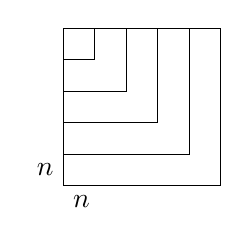
\begin{tikzpicture}
                \draw (0,0) -- (2,0) -- (2,2) -- (0,2) -- (0,0);
                \draw (0,0.4) -- (1.6,0.4) -- (1.6,2) -- (0,2) -- (0,0);
                \draw (0,0.8) -- (1.2,0.8) -- (1.2,2) -- (0,2) -- (0,0); 
                \draw (0,1.2) -- (0.8,1.2) -- (0.8,2) -- (0,2) -- (0,0) node[above left]{$n$};
                \draw (0,1.6) -- (0.4,1.6) -- (0.4,2) -- (0,2) -- (0,0) node[below right]{$n$};
            \end{tikzpicture}
        \end{center}

        This means that the determinant of the matrix obtained by taking the first $k$ rows and columns of $S$ is positive, $\forall k = 1, \dots, n$.
    \end{multicols}

    \item Cholesky decomposition: $S = B^\intercal B$, with $B$ upper triangular
    \item All pivot elements are positive in the Gaussian elimination process
\end{enumerate}

\paragraph{Proof that a Symmetric matrix is Positive Definite}
Since \(\underline{x}\) is an eigenvector and \(\underline{v}\) is a generic vector, we express \(\underline{v}\) as a linear combination of the eigenvectors of \(S\):
\[
\underline{v} = c_1 \underline{x}_1 + c_2 \underline{x}_2 + \dots + c_n \underline{x}_n
\]
Then,
\[
(c_1 \underline{x}_1 + c_2 \underline{x}_2 + \dots + c_n \underline{x}_n)^\intercal S (c_1 \underline{x}_1 + c_2 \underline{x}_2 + \dots + c_n \underline{x}_n)
\]
Expanding this, we get two types of components:
\[
\begin{cases}
c_1^2 \underline{x}_1^\intercal S \underline{x}_1 = c_1^2 \lambda_1 \|\underline{x}_1\|^2\\
c_1 c_2 \underline{x}_1^\intercal S \underline{x}_2 = c_1 c_2 \lambda_2 \underline{x}_1^\intercal \underline{x}_2 = 0 \text{ (orthogonal)}
\end{cases}
\]

This shows that \(S\) is positive semi-definite

This property can also be proved from \textit{iv}):
\[
    S = B^\intercal B \implies \underline{v}^\intercal(B^\intercal B)\underline{v} = (\underline{v}^\intercal B^\intercal)(B \underline{v}) = (B\underline{v})^\intercal (B\underline{v}) = ||B\underline{v}||^2 \geq 0   
\]